
\begin{figure}[hbt!]
	\caption{Leftmost Stock Price Digit and Probability of Sale, Quarterly Sample}%
	\label{fig:left_digit_sell_main}%
	\centering%	
	\bigskip
	\subfigure[Price Increasing]{
		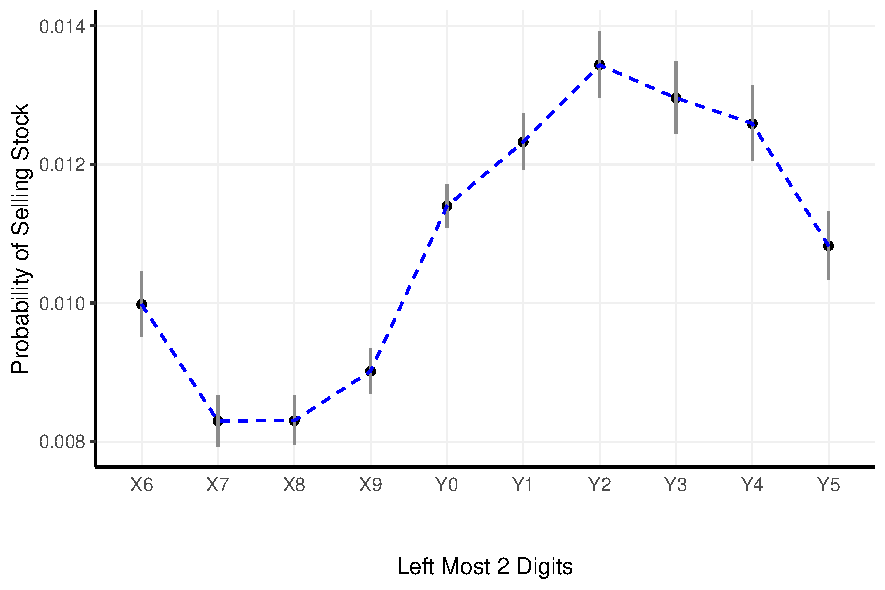
\includegraphics[width=0.45\textwidth]{figures/Left2increase_probCI_quarter.pdf}
		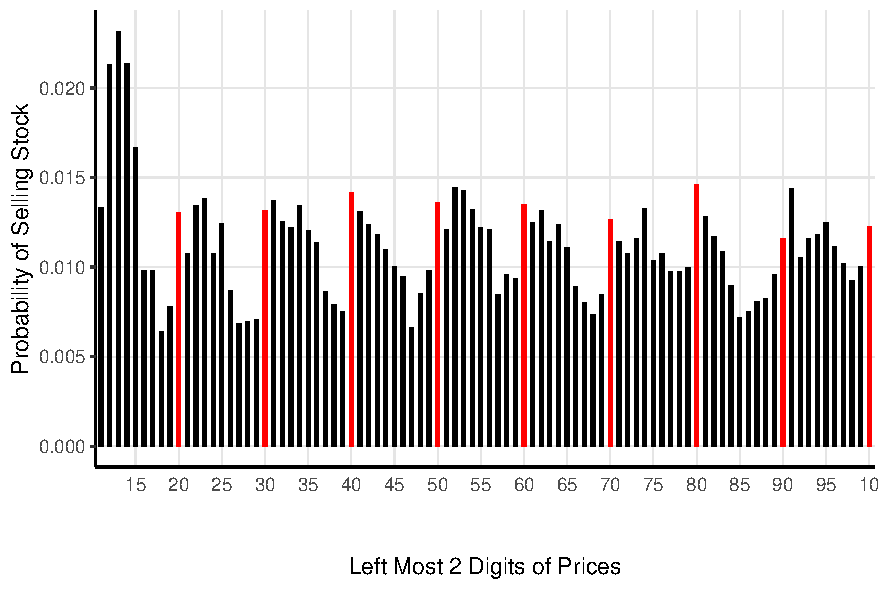
\includegraphics[width=0.45\textwidth]{figures/2left_increase_quarter.pdf}	
	}
	\subfigure[Price Decreasing]{
		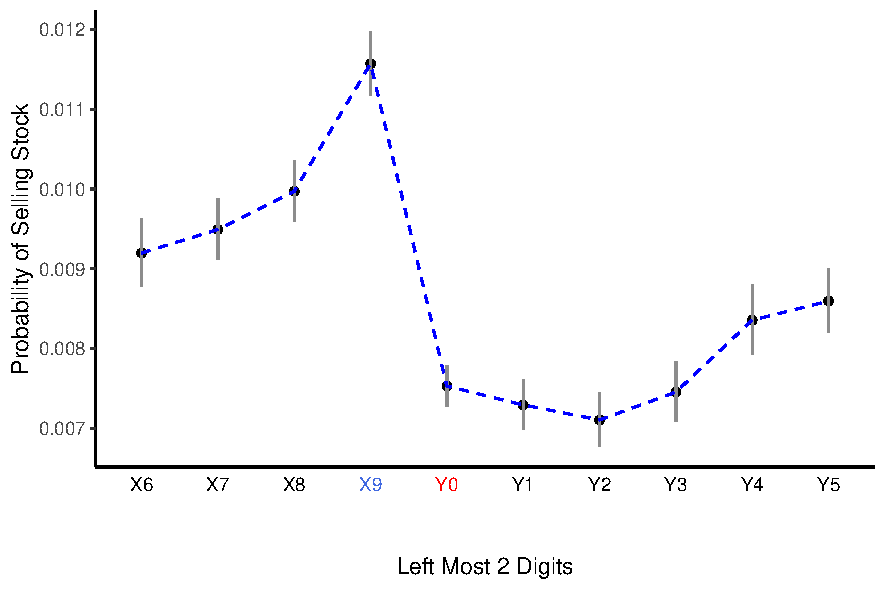
\includegraphics[width=0.45\textwidth]{figures/Left2decrease_probCI_quarter.pdf}
		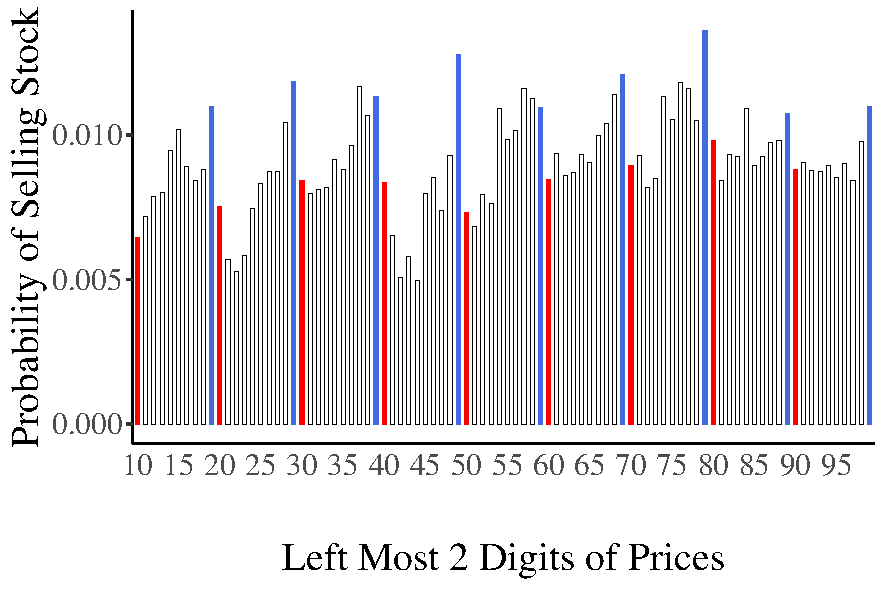
\includegraphics[width=0.45\textwidth]{figures/2left_decrease_quarter.pdf}	
	}
	\fignote{£$Y$ in the X-axes is equivalent to £$X+1$ (e.g., £X9 could include £0.19, £1.9, £19, etc., while £Y0 could include £0.20, £2.0, £20, etc.).}
\end{figure}

\clearpage

\begin{figure}[hbt!]
	\caption{Leftmost Stock Price Digit and Probability of Sale \\ Prices Increasing Sample by Price Range}%
	\label{fig:left_digit_sell_increase_main}%
	\centering%	
	\bigskip
	\subfigure[Price = \pounds0.11 to \pounds1.01]{
		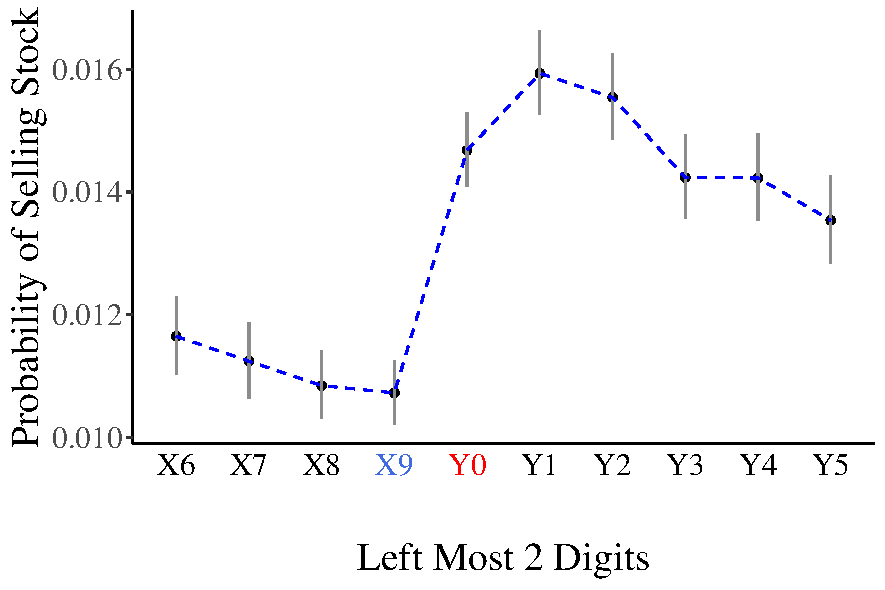
\includegraphics[width=0.45\textwidth]{figures/Left2increases_1pbin_CI_quarter.pdf}
		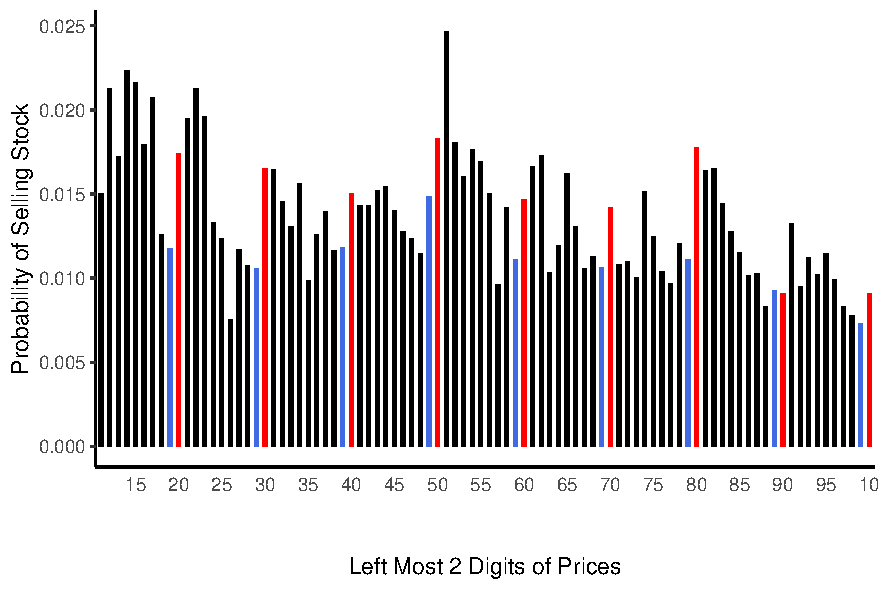
\includegraphics[width=0.45\textwidth]{figures/2left_increase_bin1p_quarter.pdf}
	}
	\subfigure[Price = \pounds1.01 to \pounds10.1]{
		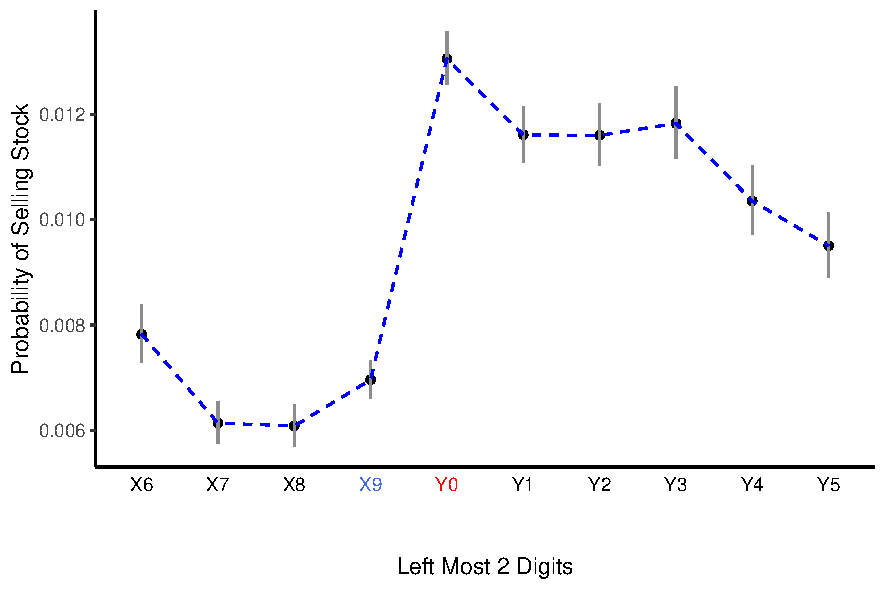
\includegraphics[width=0.45\textwidth]{figures/Left2increases_10pbin_CI_quarter.pdf}
		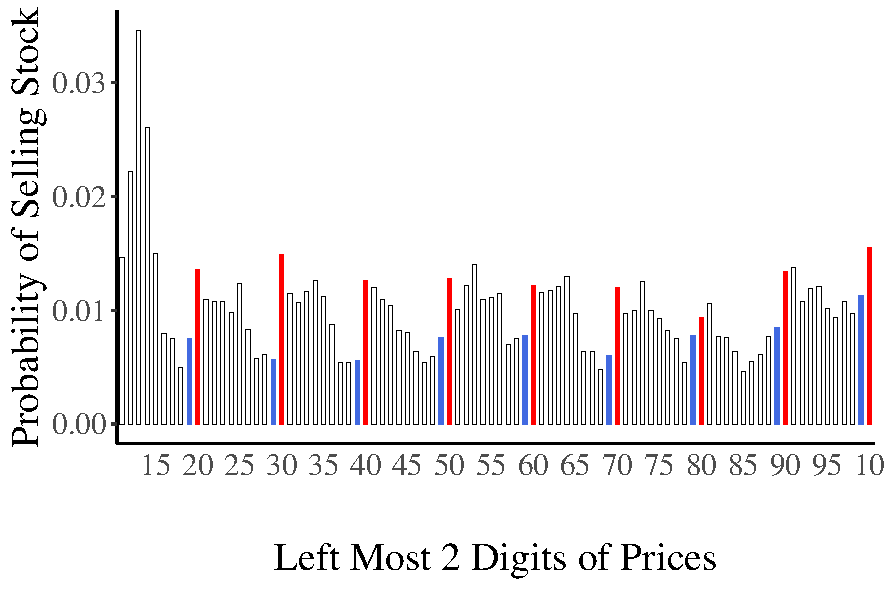
\includegraphics[width=0.45\textwidth]{figures/2left_increase_bin10p_quarter.pdf}
	}
	\subfigure[Price = \pounds11 to \pounds101]{
		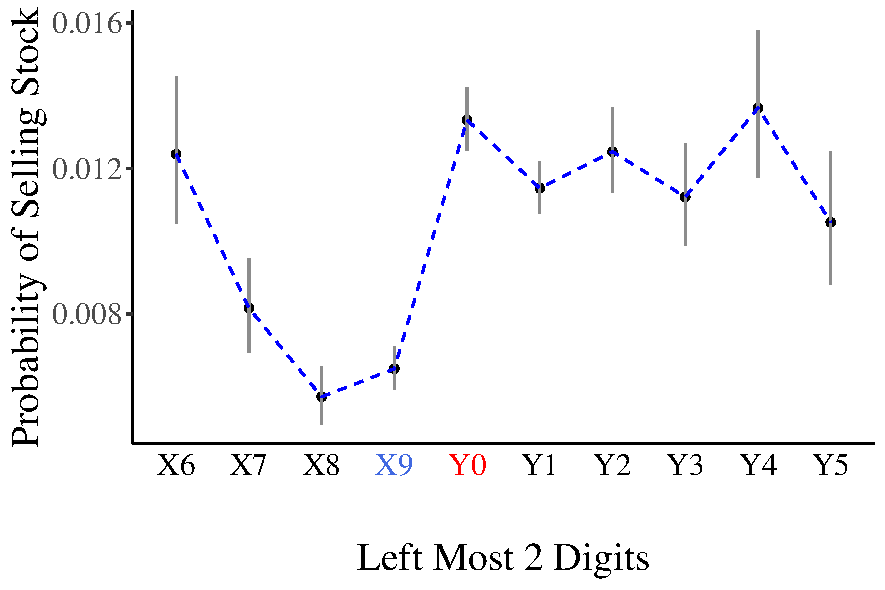
\includegraphics[width=0.45\textwidth]{figures/Left2increases_1poundbin_CI_quarter.pdf}
		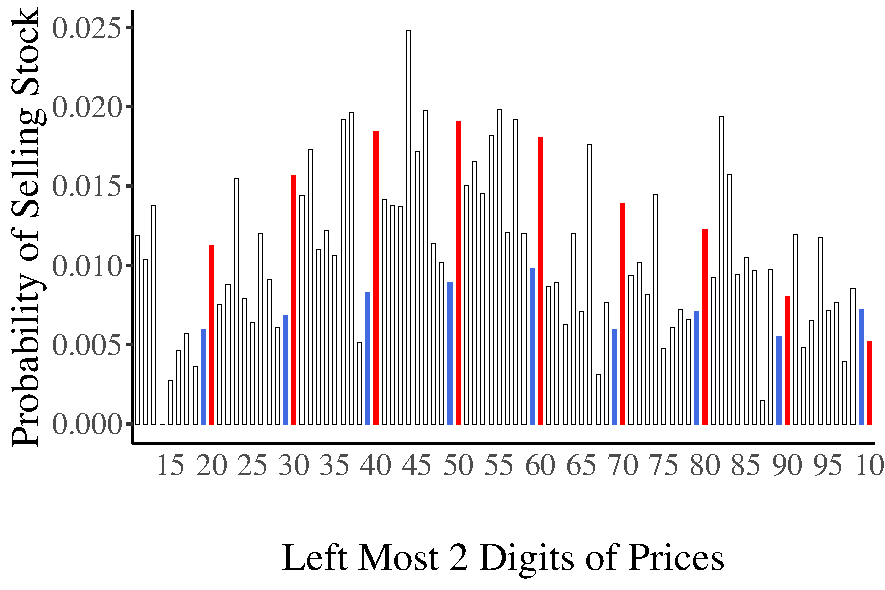
\includegraphics[width=0.45\textwidth]{figures/2left_increase_bin1pound_quarter.pdf}
	}
	\fignote{£$Y$ in the X-axes is equivalent to £$X+1$ (e.g., £X9 could include £0.19, £1.9, £19, etc., while £Y0 could include £0.20, £2.0, £20, etc.). Panels A, B and C show equal size bins of 1p, 10p and £1, respectively. Panel A corresponds to 25\% of the observations in the prices increasing sample; Panel B, to 55\%; and Panel C, to 7\%.}
\end{figure}

\clearpage
\begin{figure}[hbt!]
	\caption{Leftmost Stock Price Digit and Probability of Sale \\ Prices Decreasing Sample by Price Range}%
	\label{fig:left_digit_sell_decrease_main}%
	\centering%	
	\bigskip
	\subfigure[Price = \pounds0.10 to \pounds1.00]{
		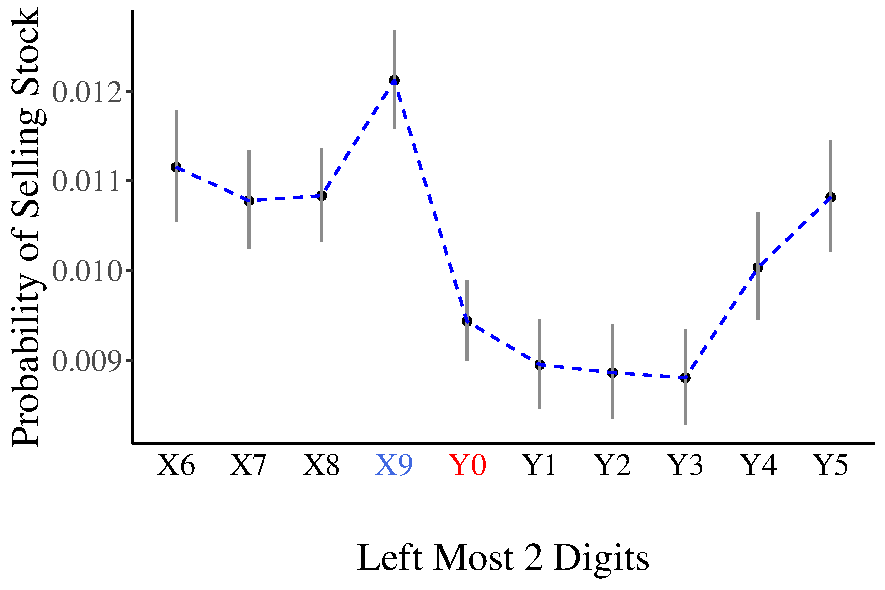
\includegraphics[width=0.45\textwidth]{figures/Left2decreases_1pbin_CI_quarter.pdf}
		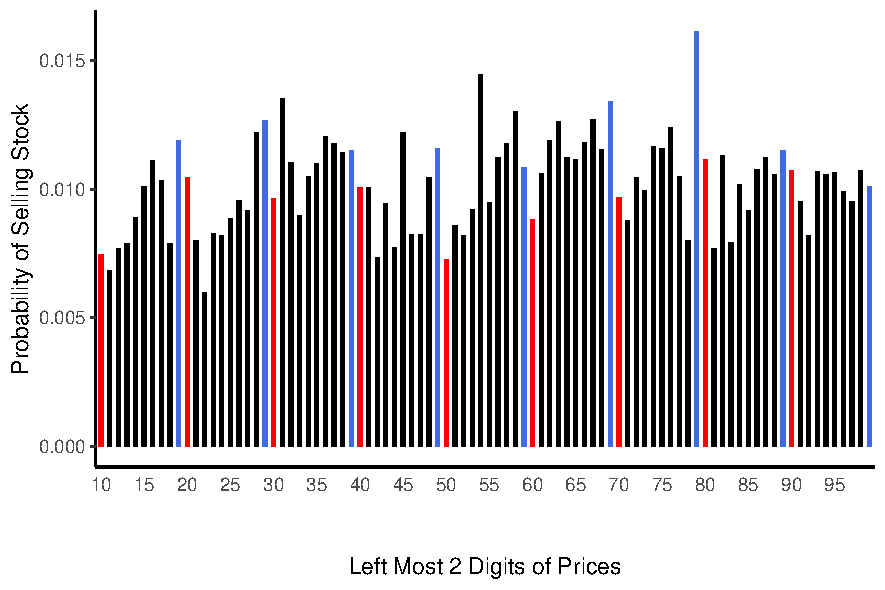
\includegraphics[width=0.45\textwidth]{figures/2left_decrease_bin1p_quarter.pdf}
	}
	\subfigure[Price = \pounds1.00 to \pounds10.0]{
		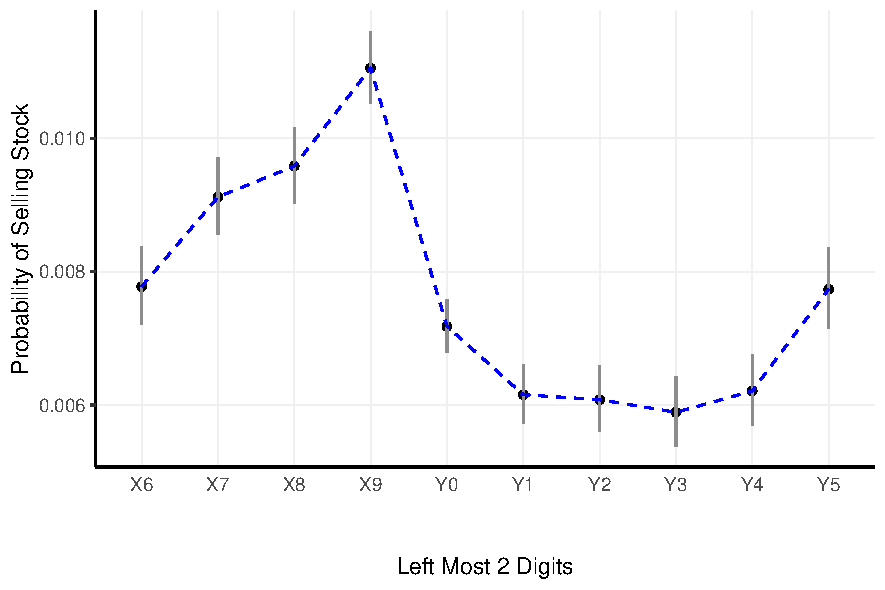
\includegraphics[width=0.45\textwidth]{figures/Left2decreases_10pbin_CI_quarter.pdf}
		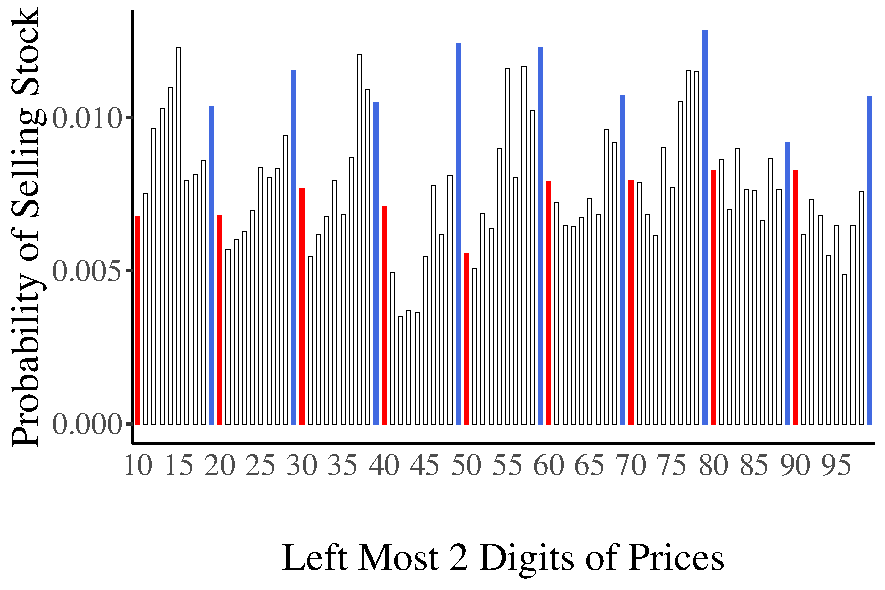
\includegraphics[width=0.45\textwidth]{figures/2left_decrease_bin10p_quarter.pdf}
	}
	\subfigure[Price = \pounds10 to \pounds100]{
		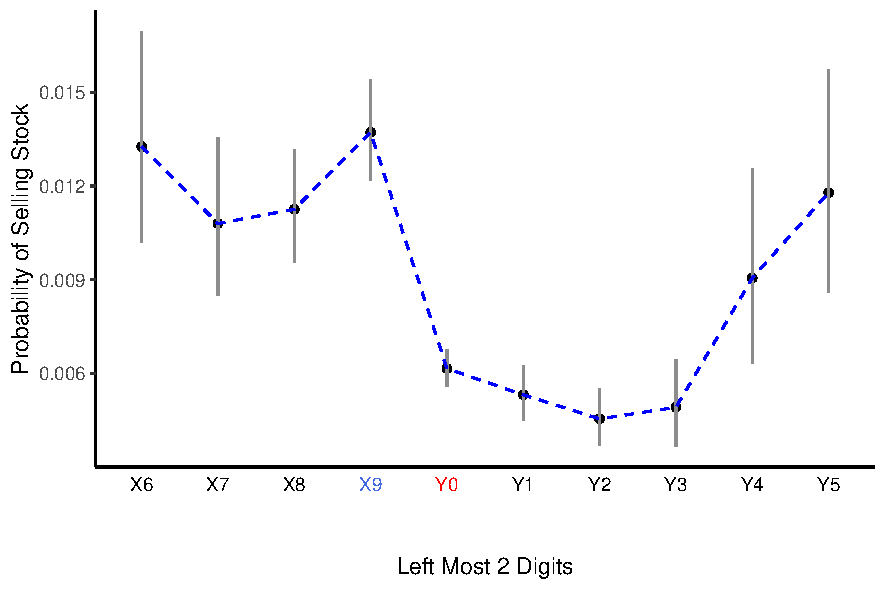
\includegraphics[width=0.45\textwidth]{figures/Left2decreases_1poundbin_CI_quarter.pdf}
		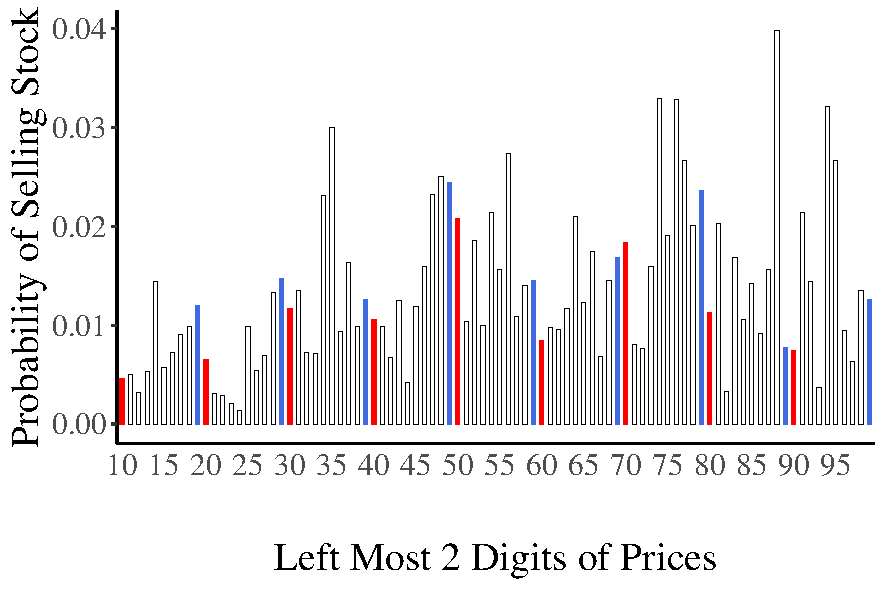
\includegraphics[width=0.45\textwidth]{figures/2left_decrease_bin1pound_quarter.pdf}
	}
	\fignote{£$Y$ in the X-axes is equivalent to £$X+1$ (e.g., £X9 could include £0.19, £1.9, £19, etc., while £Y0 could include £0.20, £2.0, £20, etc.). Panels A, B and C show equal size bins of 1p, 10p and £1, respectively. Panel A corresponds to 27\% of the observations in the prices decreasing sample; Panel B, to 44\%; and Panel C, to 7\%.}
\end{figure}

\clearpage

\begin{figure}[hbt!]
	\caption{Leftmost Stock Price Digit and Probability of Sale, \\ Prices Increasing Sample Limit Order Robustness Tests}%
	\label{fig:limit_order_figures}%
	\centering%	
	\bigskip
	\subfigure[Excluding Pre-Market and After-Hours Sells (Outside 8am to 4:30pm)]{	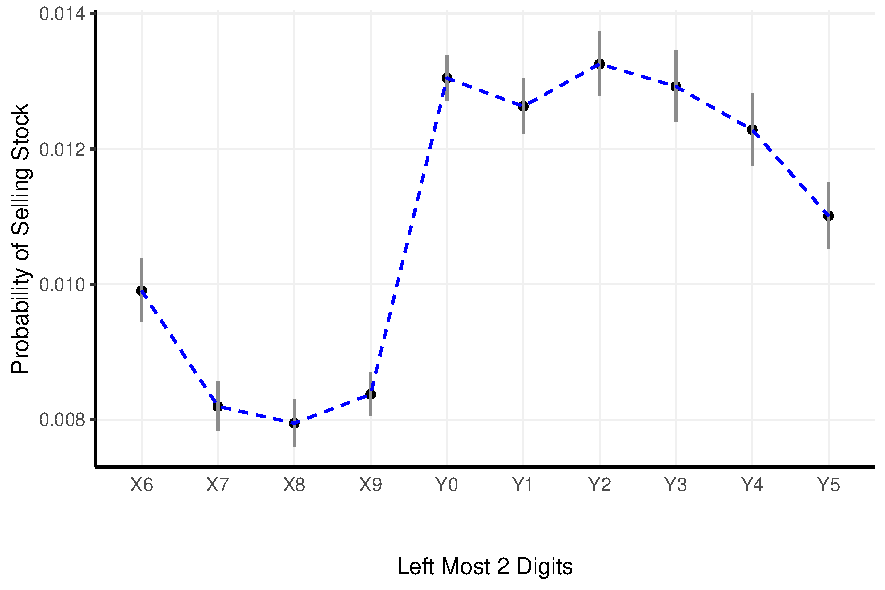
\includegraphics[width=0.4\textwidth]{figures/outside_hoursLeft2increase_probCI_quarter.pdf}
	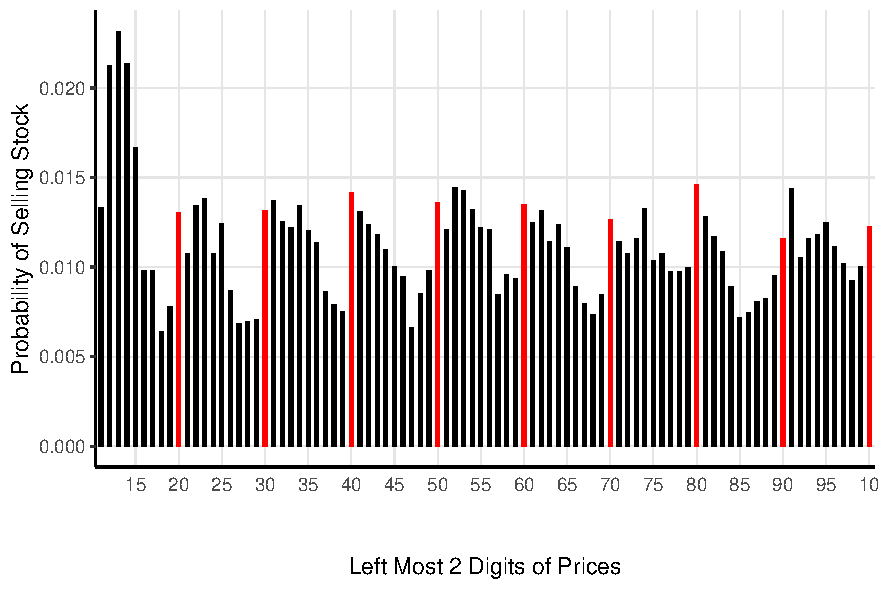
\includegraphics[width=0.4\textwidth]{figures/outside_hours2left_increase_quarter.pdf}	
	}
	\subfigure[Excluding Sells with Login the Day Before or Weekend Logins for Monday Sells]{
		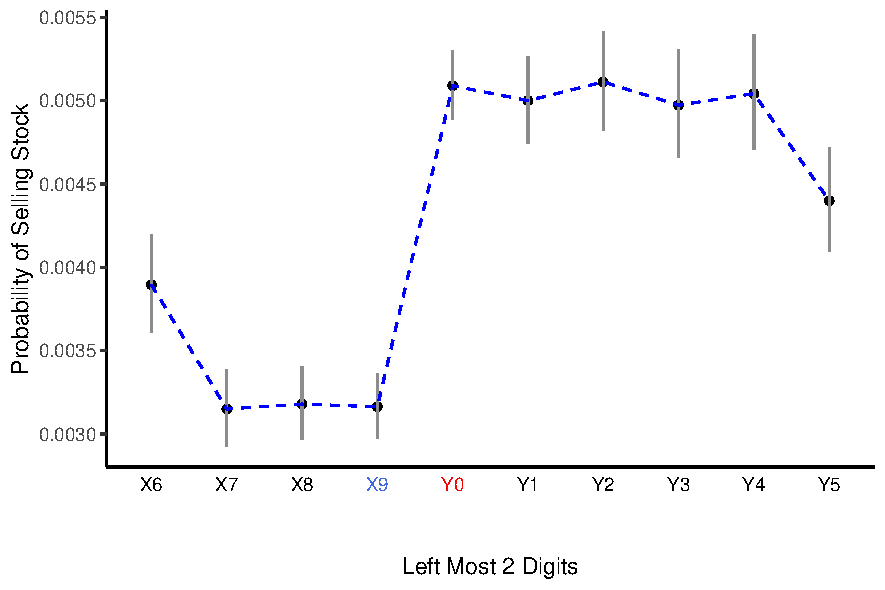
\includegraphics[width=0.4\textwidth]{figures/no_yest_loginLeft2increase_probCI_quarter.pdf}
		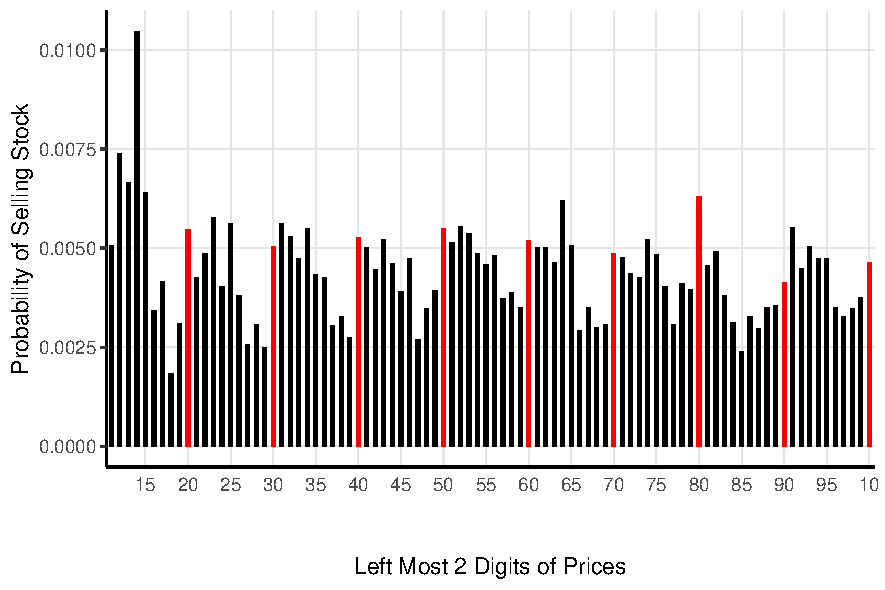
\includegraphics[width=0.4\textwidth]{figures/no_yest_login2left_increase_quarter.pdf}
	}
	\subfigure[Including Only FTSE100 Stocks]{
		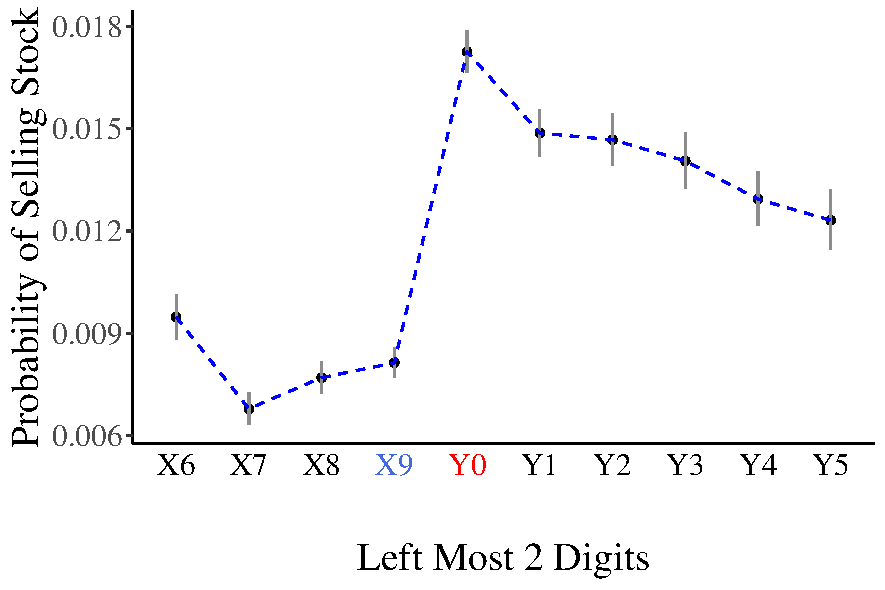
\includegraphics[width=0.4\textwidth]{figures/liquidLeft2increase_probCI_quarter.pdf}
		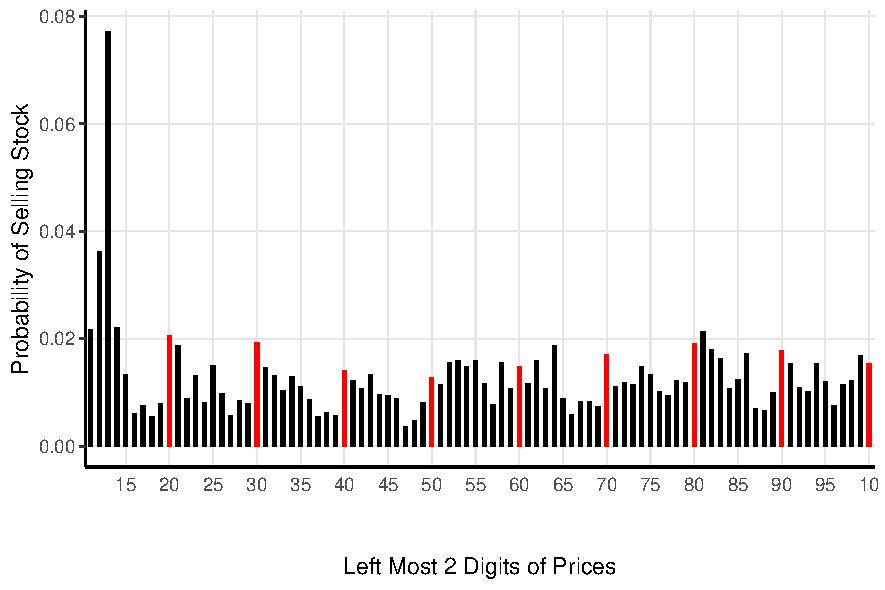
\includegraphics[width=0.4\textwidth]{figures/liquid2left_increase_quarter.pdf}		}
	\subfigure[Excluding Accounts with Potential Limit Orders (Linnainmaa, 2010)]{
		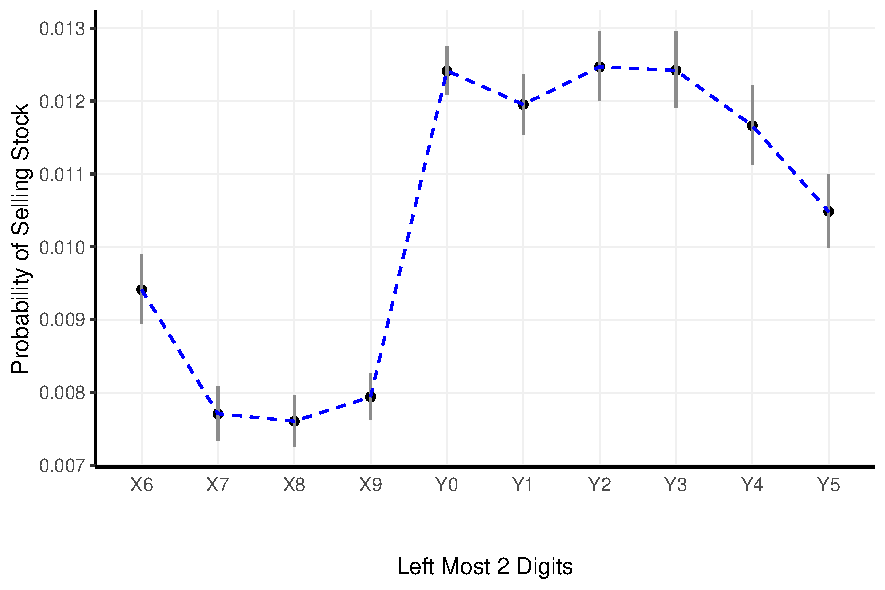
\includegraphics[width=0.4\textwidth]{figures/potential_lmLeft2increase_probCI_quarter.pdf}
		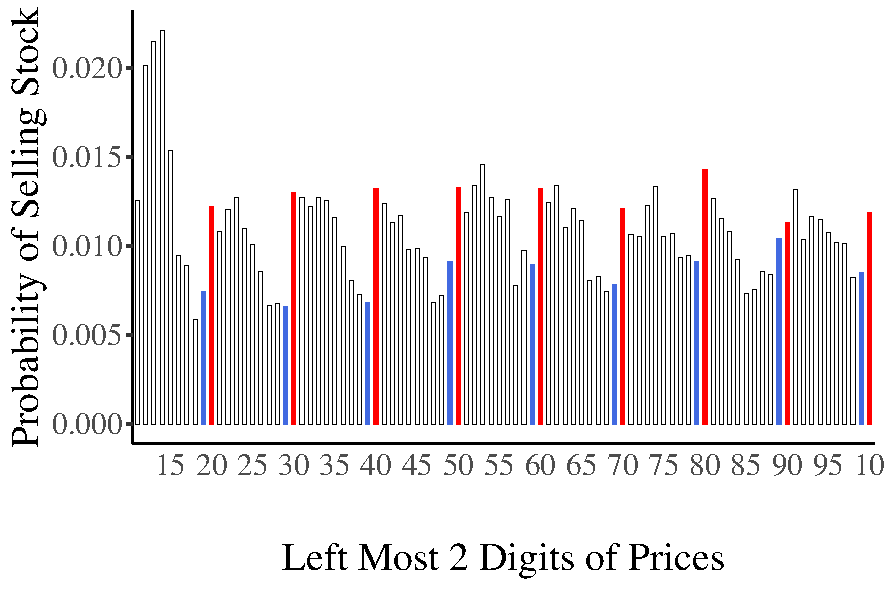
\includegraphics[width=0.4\textwidth]{figures/potential_lm2left_increase_quarter.pdf}
	}
	\fignote{£$Y$ in the X-axes is equivalent to £$X+1$ (e.g., £X9 could include £0.19, £1.9, £19, etc., while £Y0 could include £0.20, £2.0, £20, etc.).  Panels display different sample restrictions to exclude sells corresponding to limit orders. Panel A drops sells executed when the market was closed. It also exclude potential discretionary trades (high frequency trades executed on the same stock, at the same time and at the same price that would likely correspond to sells arranged by Barclays discretionary service). Panel B excludes sells with a preceding login day. Panel C exclude non-liquid stocks, and Panel D excludes potential limit orders following Linnainmaa (2010) methodology. Panel A drops 2.2\% of sells, Panel B drops 64.7\% of sells, Panel C drops 75.9\% of sells, and Panel D drops 11.4\% of sells.} 
\end{figure}

\clearpage
\begin{figure}[hbt!]
	\caption{Distribution of Individual Left Digit Bias Coefficient Estimates}%
	\label{fig:hist_ind_betas}%
	\centering%	
	\bigskip
	\subfigure[Price Increasing Sample]{
		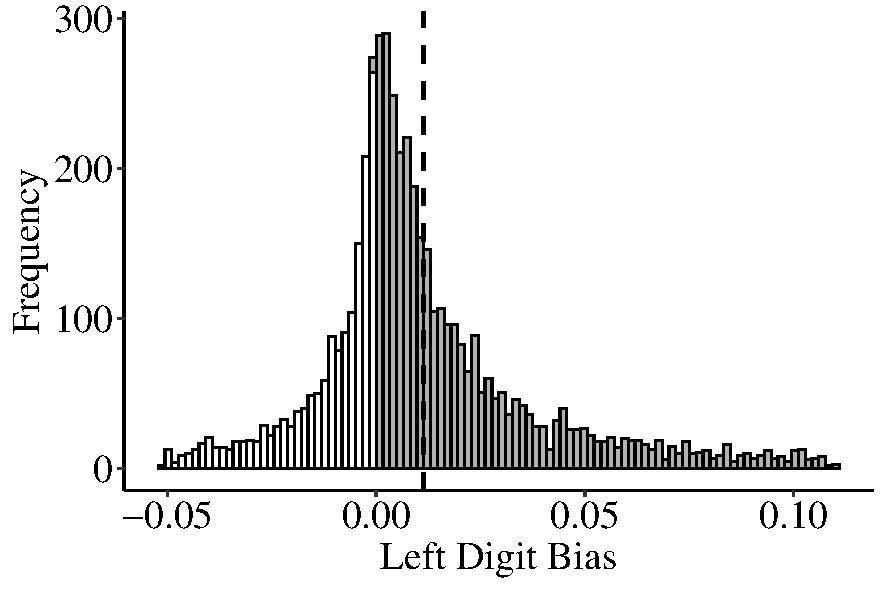
\includegraphics[width=0.6\textwidth]{figures/hist_betas_increasing.pdf}
	}
	\subfigure[Price Decreasing Sample]{
		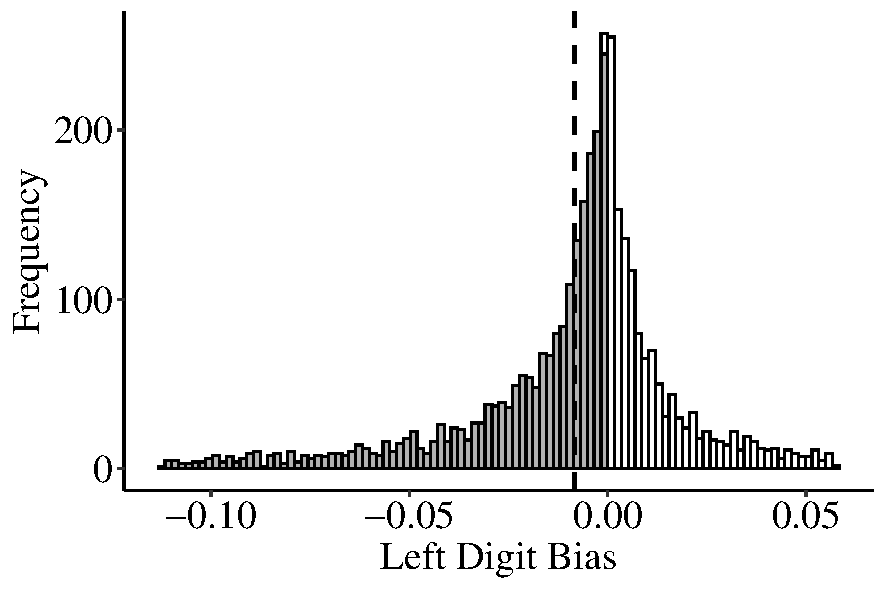
\includegraphics[width=0.6\textwidth]{figures/hist_betas_decreasing.pdf}	
	}
	\fignote{The histograms plot the distribution of the coefficients for the dummy \textit{Above Y0=1} (or left digit bias) for each account in the aggregate of price increasing samples (including the monthly, quarterly and annual samples) (left panel) and the aggregate of price decreasing samples (right panel). The dashed line reflects the mean of the distributions. Only accounts displaying at least 5 sells in the data are included (4,987 accounts in the left panel and 3,544 in the right panel). Outliers below the 5 percentile and above the 95 percentile are excluded.}
\end{figure}

